%%%%%%%%%%%%%%%%%%%%%%%%%%%%%%%%%%%%%%%%%%%%%%%%%%%%%%%%%%%%%%%%%%%%%%%%%%%%%%%%
\chapter{Analysis of Affymetrix Microarrays}
\label{ch:affy}
%%%%%%%%%%%%%%%%%%%%%%%%%%%%%%%%%%%%%%%%%%%%%%%%%%%%%%%%%%%%%%%%%%%%%%%%%%%%%%%%

Affymetrix GeneChip arrays are considered the industry standard in terms of
high-density oligonucleotide microarrays. In this chapter, we analyze the layout
of several GeneChip arrays with respect to the quality measures defined in
Chapter \ref{ch:mlp}, i.e., border length and conflict index. We then use some
of the algorithms presented in previous chapters to create alternative layouts
for two commercially available microarrays.

%%%%%%%%%%%%%%%%%%%%%%%%%%%%%%%%%%%%%%%%%%%%%%%%%%%%%%%%%%%%%%%%%%%%%%%%%%%%%%%%
\section{Introduction}
\label{sec:affy_intro}

We obtained the specification of several GeneChip arrays containing the list of
probe sequences and their positions on the chip from Affymetrix's web
site\footnote{\url{http://www.affymetrix.com/support/technical/byproduct.affx?cat=arrays}}.
As discussed below, we have to make a few assumptions because some details such
as the deposition sequence used to synthesize the probes, the probe embeddings,
and the contents of ``special'' spots are not publicly available.

Some of the special spots are used to help the mechanical alignment of the chip
with the scanner that captures the image with the hybridization signals. Others
contain \emph{quality control probes} used to detect failures during the
production of the chip \citep{Affymetrix2002,Hubbell1999a}. Not knowing the
contents of these special spots did not interfere with our analysis because, in
all arrays we examined, they amount to at most $1.22\%$ of the total number of
spots.

What could interfere with our analysis is the fact that some arrays have a
significant number of empty spots (as much as $11.94\%$ on the Chicken Genome
array). The physical location of some empty spots suggest that they might be
used as ``spacers'' to separate regions of the chip. Others might be empty
simply because the number of spots exceeds the number of probes. A high number
of empty spots result in a relatively low normalized border length (as defined
in Section \ref{sec:mlp_bl_vs_ci}) since we divide the total number of border
conflicts by the number of internal borders of the chip (an empty spot
contributes to the number of internal borders but obviously not to the number of
border conflicts). Thus, to better compare chips with different amounts of empty
spots we also use the \emph{average number of border conflicts per probe},
defined as the total border length divided by the number of probes. As we shall
see, an array with many empty spots might still have an advantage depending on
how the empty spots are distributed on the chip.

It has been reported that a fixed 74-step deposition sequence is used by
Affymetrix \citep{Kahng2004}. An analysis with the algorithms presented in
Chapter \ref{ch:scs} revealed that all GeneChip arrays, regardless of their
size, can be synthesized in $N=(\Seq{TGCA})^{18}\Seq{TG}$, i.e., $18.5$ cycles
of \Seq{TGCA}, and that a shorter deposition sequence is indeed unlikely. This
suggests that only sub-sequences of this particular deposition sequence can be
used as probes on Affymetrix chips. In principle, this should not be a problem
as this sequence covers about $98.45\%$ of all 25-mers \citep{Rahmann2006}.

\begin{figure}[t]\centering
\begin{tabular}{lc}
$N$              & \footnotesize{\tt{\verb|TGCATGCATGCATGCATGCATGCATGCATGCATGCATGCATGCATGCATGCATGCATGCATGCATGCATGCATG|}} \\
\hline
$\eps_p$         & \footnotesize{\tt{\verb| G AT   TG A G A   A  C   C  GCA G  T  A  C  G A  C   C   C  G  T         |}} \\
$\eps_{\bar{p}}$ & \footnotesize{\tt{\verb| G AT   TG A G A   A  C   C  G   G A G  T  A  C  G A  C   C   C  G  T     |}} \\
                 & \footnotesize{\tt{\verb|                              ++   +++ ++ ++ +++ +++         ++ ++  +     |}} \\
\hline
$\eps_p$         & \footnotesize{\tt{\verb| G AT   TG A G A   A  C   C  GC    A G  T  A  C  G A  C   C   C  G  T     |}} \\
$\eps_{\bar{p}}$ & \footnotesize{\tt{\verb| G AT   TG A G A   A  C   C  G   G A G  T  A  C  G A  C   C   C  G  T     |}} \\
                 & \footnotesize{\tt{\verb|                              +  +                                        |}} \\
\hline
\end{tabular}
\caption{\label{fig:pairwise_leftmost}%
  Left-most (above) and pair-wise left-most (below) embeddings $\eps_p$ and
  $\eps_{\bar{p}}$ of perfect match (PM) and mismatch (MM) probes
  $p=\Seq{GATTGAGAACCGCAGTACGACCCGT}$ and
  $\bar{p}=\Seq{GATTGAGAACCGGAGTACGACCCGT}$, respectively, in the standard
  Affymetrix deposition sequence $N=(\Seq{TGCA})^{18}\Seq{TG}$. Conflicts
  between the embeddings are highlighted with plus signs (\small{\tt{+}})
  in the corresponding synthesis steps.}
\end{figure}

Probes of GeneChip arrays always appear in pairs: the perfect match (PM), which
perfectly matches its target sequence, and the mismatch (MM) probe, which is
used to quantify cross-hybridizations and unpredictable background signal
variations \citep{Affymetrix2001}. The MM probe is a copy of the PM probe except
for the middle base (position 13 of the 25-mer), which is exchanged with its
Watson-Crick complement. The layout of GeneChip arrays alternate rows of PM
probes with rows of MM probes in such a way that probes of a pair are always
adjacent on the chip. Moreover, PM and MM probes are \emph{pair-wise left-most
embedded} \citep{Kahng2004}. Informally, a pair-wise left-most embedding is
obtained from left-most embeddings by shifting the second half of one embedding
to the right until the two embeddings are ``aligned'' in the synthesis steps
that follow the mismatched middle bases (Figure \ref{fig:pairwise_leftmost}).
This approach reduces border conflicts between the probes of a pair, although it
leaves a conflict in the steps that add the middle bases.

The fact that probes must appear in pairs restricts even more which sequences
can be used as probes on GeneChip arrays because both PM and MM probes must
``fit'' in the deposition sequence. For example, although
$p=\Seq{CGTAGGTACGTTATAAGTCACTAAA}$ has an embeddeding in
$N=(\Seq{TGCA})^{18}\Seq{TG}$, it cannot be used as a probe because its
corresponding mismatch probe $\bar{p}=\Seq{CGTAGGTACGTTTTAAGTCACTAAA}$ cannot be
embedded in $N$, as shown below.

\begin{tabular}{lc}
$N$              & \footnotesize{\tt{\verb|TGCATGCATGCATGCATGCATGCATGCATGCATGCATGCATGCATGCATGCATGCATGCATGCATGCATGCATG  |}} \\
\hline
$\eps_p$         & \footnotesize{\tt{\verb|  C  G  T  A G   G  T  A  C  G  T   T  AT  A   A G  T CA  C T  A   A   A    |}} \\
$\eps_{\bar{p}}$ & \footnotesize{\tt{\verb|  C  G  T  A G   G  T  A  C  G  T   T   T   T  A   A G  T CA  C T  A   A   A|}} \\
\hline
\end{tabular}

%%%%%%%%%%%%%%%%%%%%%%%%%%%%%%%%%%%%%%%%%%%%%%%%%%%%%%%%%%%%%%%%%%%%%%%%%%%%%%%%
\section{Layout Analysis}
\label{sec:affy_analysis}

\begin{figure}[t]\centering
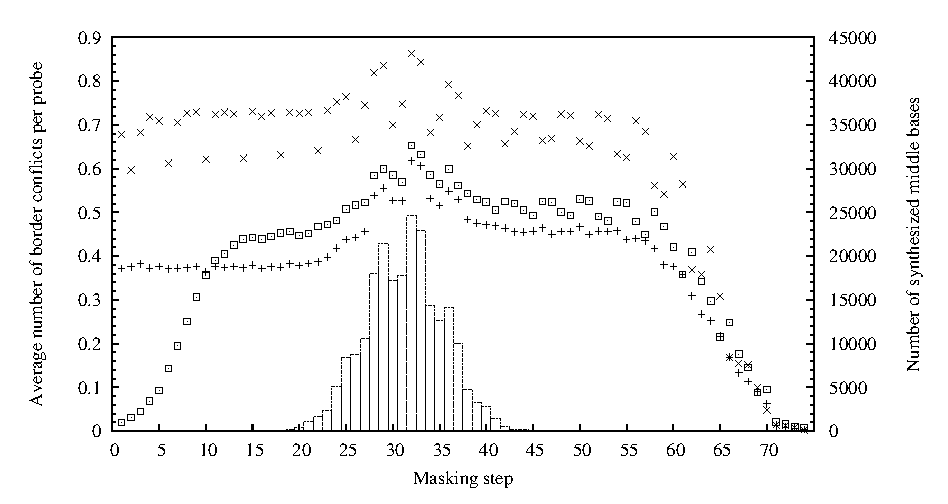
\includegraphics{affy/genechip/affy_blm}
\caption{\label{fig:affy_blm}%
  Average number of border conflicts per probe per masking step (on the left
  y-axis) of three GeneChip arrays, assuming pair-wise left-most embeddings:
  Yeast Genome S98 ({\scriptsize $\times$}), Human Genome U95A2 ({\tiny $+$}),
  and E.\ coli Genome 2.0 ({\tiny $\boxdot$}). The number of middle bases
  synthesized at each step on the E.\ coli Genome 2.0 is shown in boxes (on the
  right y-axis).}
\end{figure}

Figure \ref{fig:affy_blm} shows the average number border conflicts per probe
per masking step of three GeneChip arrays. We assume that the probes are
pair-wise left-most embedded in $N=(\Seq{TGCA})^{18}\Seq{TG}$, and we consider
all spots whose contents are not available as empty spots. In all chips we
analyzed, the number of border conflicts are higher in the steps that add the
middle bases, a result of placing PM and MM probes in adjacent spots. The Yeast
Genome S98 array has the worst layout in terms of border conflicts and most of
the earlier GeneChip arrays such as the E.\ coli Antisense Genome have similar
levels of conflicts. The layout of the Human Genome U95A2 array has signficantly
less border conflicts than the Yeast array, suggesting that it was designed with
a better placement strategy. The curve of the E.\ coli Genome 2.0 array, with
very low levels of conflicts in the first 10 masks, is typical of the latest
generation of GeneChip arrays, including the Chicken Genome and the Wheat Genome
(one of the largest GeneChip arrays currently available with
$1\,164\times 1\,164$ spots), and suggest yet another placement strategy.

Figure \ref{fig:ecoli_masks} shows a representation of selected masks for the
E.\ coli Genome 2.0. The low levels of conflicts in the first synthesis steps
are a result of the pattern of masked and unmasked layers that can be seen in
masks $M_1$ to $M_9$. This pattern is similar to the ones produced by Greedy
(Figure \ref{fig:greedy-bl_masks}) and \Greedyplus\ (Figure
\ref{fig:gplus-bl_masks}). A more careful examination, however, reveals that the
layers are arranged in a way that resembles the Gray-code--based arrangement
employed by 1-Dimensional Partitioning (Figure \ref{fig:1dpart}). This does not
necessarily mean that the layout was produced by such a partitioning. In fact, a
similar effect could be produced by a placement algorithm such as Greedy or
\Greedyplus\ if the probes were ordered in such a way that a prefix of their
binary embeddings formed an approximation of a Gray code.

\begin{figure}[p]\centering
%%
\begin{picture}(435,567)\footnotesize{
\put( -2,439){\makebox(145,128){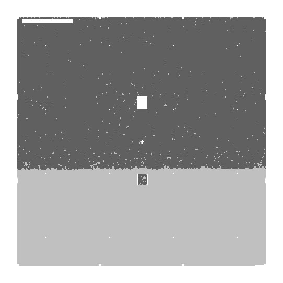
\includegraphics{affy/genechip/mask01}}}
\put(147,439){\makebox(145,128){
\includegraphics{affy/genechip/mask02}}}
\put(292,439){\makebox(145,128){
\includegraphics{affy/genechip/mask03}}}
\put( -2,429){\makebox(145, 10){$M_1$}}
\put(147,429){\makebox(145, 10){$M_2$}}
\put(292,429){\makebox(145, 10){$M_3$}}
\put( -2,296){\makebox(145,128){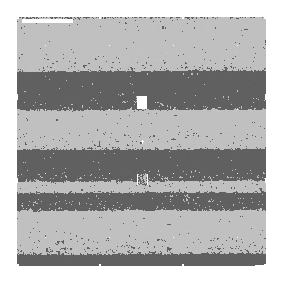
\includegraphics{affy/genechip/mask04}}}
\put(147,296){\makebox(145,128){
\includegraphics{affy/genechip/mask05}}}
\put(292,296){\makebox(145,128){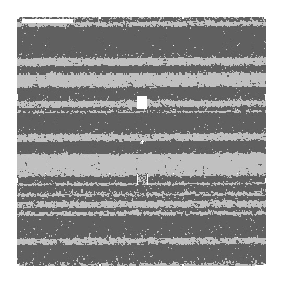
\includegraphics{affy/genechip/mask06}}}
\put( -2,286){\makebox(145, 10){$M_4$}}
\put(147,286){\makebox(145, 10){$M_5$}}
\put(292,286){\makebox(145, 10){$M_6$}}
\put( -2,153){\makebox(145,128){
\includegraphics{affy/genechip/mask07}}}
\put(147,153){\makebox(145,128){
\includegraphics{affy/genechip/mask08}}}
\put(292,153){\makebox(145,128){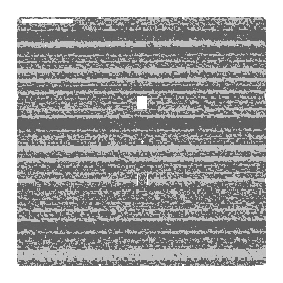
\includegraphics{affy/genechip/mask09}}}
\put( -2,143){\makebox(145, 10){$M_7$}}
\put(147,143){\makebox(145, 10){$M_8$}}
\put(292,143){\makebox(145, 10){$M_9$}}
\put( -2, 10){\makebox(145,128){
\includegraphics{affy/genechip/mask32}}}
\put(147, 10){\makebox(145,128){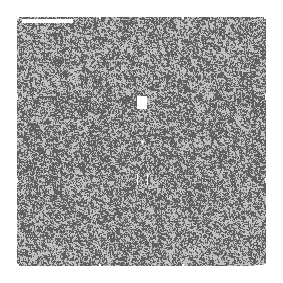
\includegraphics{affy/genechip/mask50}}}
\put(292, 10){\makebox(145,128){
\includegraphics{affy/genechip/mask70}}}
\put( -2,  0){\makebox(145, 10){$M_{32}$}}
\put(147,  0){\makebox(145, 10){$M_{50}$}}
\put(292,  0){\makebox(145, 10){$M_{70}$}}
}\end{picture}
%%
\caption{\label{fig:ecoli_masks}%
  Selected masks of Affymetrix's E.\ coli Genome 2.0 GeneChip array, assuming
  pair-wise left-most embeddings. Unmasked (masked) spots are represented by
  light (dark) dots. White regions represent spots whose contents are not
  publicly available.}
\end{figure}

Table \ref{tab:genechip} confirms that the layout of the Human Genome U95A2
array is the best in terms of normalized border length and average conflict
index. This, however, has more to do with empty spots than with the placement
strategy as this chip has about $1.83\%$ of empty spots that are evenly
distributed on the chip surface (Figure \ref{fig:chipmaps}, left). In contrast,
the Chicken Genome array has an exceptionally high percentage of empty spots
($11.94\%$) that contribute to lower the normalized border length but that does
not result in a lower average number of border conflicts per probe in comparison
with the Human Genome array because the empty spots are concentrated in the
lower part of the chip (Figure \ref{fig:chipmaps}, right).

\begin{table}[t!]\centering
\caption{\label{tab:genechip}
  Average number of border conflicts per probe (ABC), normalized border length
  (NBL) and average conflict index (ACI) of selected GeneChip arrays (assuming
  pair-wise left-most embeddings). The dimension of the chip, the percentage of
  spots with unknown content and the percentage of empty spots are also shown.}
\footnotesize{
\begin{tabular}{lcrrrrr}
GeneChip Array            & Dimension             & Unknown  & Empty     & ABC     & NBL     & ACI \\
\hline
Yeast Genome S98          & $534\times 534$       & $1.22\%$ &  $1.70\%$ & 44.8168 & 21.7945 & 669.0663 \\
E.\ coli Antisense Genome & $544\times 544$       & $1.17\%$ &  $3.12\%$ & 43.3345 & 20.7772 & 663.7353 \\
Human Genome U95A2        & $640\times 640$       & $0.96\%$ &  $1.83\%$ & 28.2489 & 13.7517 & 510.3418 \\
E.\ coli Genome 2.0       & $478\times 478$       & $1.08\%$ &  $0.46\%$ & 29.2038 & 14.4079 & 550.2014 \\
Chicken Genome            & $984\times 984$       & $0.46\%$ & $11.94\%$ & 28.2087 & 12.3680 & 540.5022 \\
Wheat Genome              & $1\,164\times 1\,164$ & $0.38\%$ &  $0.08\%$ & 27.6569 & 13.7771 & 539.9632 \\
\hline
\end{tabular}}
\end{table}

GeneChip arrays exhibit relatively low levels of border conflicts when compared
to layouts produced by the best algorithms for random arrays of similar
dimensions. This can be explained by the fact that each probe has a nearly
identical copy next to it. Not surprisingly, these arrays have relatively high
average conflict indices when compared to random arrays because the conflicts
are concentrated on the synthesis steps that add the middle bases.

\begin{figure}[t]\centering
%%
\begin{picture}(435,225)
\put(  0, 15){\makebox(210,210){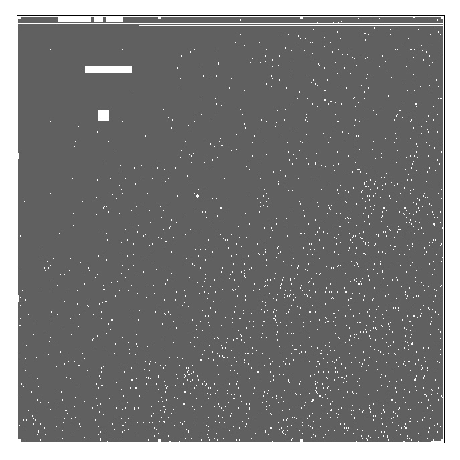
\includegraphics{affy/genechip/HGU95A2-S_affy_chipmap}}}
\put(210, 15){\makebox( 15,210){}}
\put(225, 15){\makebox(210,210){
\includegraphics{affy/genechip/CHK-S_affy_chipmap}}}
\put(  0,  0){\makebox(210, 15){\footnotesize{Human Genome U95A2 ($640\times 640$)}}}
\put(210,  0){\makebox( 15, 15){}}
\put(225,  0){\makebox(210, 15){\footnotesize{Chicken Genome ($984\times 984$)}}}
\end{picture}
%%
\caption{\label{fig:chipmaps}%
  Distribution of empty spots on two GeneChip arrays. Chip dimensions are
  indicated in parenthesis (images were scaled differently). Non-empty spots are
  represented by dark dots. White dots represent empty spots or spots whose
  contents are not publicly available.}
\end{figure}

%%%%%%%%%%%%%%%%%%%%%%%%%%%%%%%%%%%%%%%%%%%%%%%%%%%%%%%%%%%%%%%%%%%%%%%%%%%%%%%%
\section{Alternative Layouts}
\label{sec:affy_alternative}

We used \Greedyplus\ (Chapter \ref{ch:merge}) and Sequential re-embedding
(Section \ref{sec:reembed_sequential}) to create alternative layouts for two of
the latest generation of GeneChip arrays: E.\ coli Genome 2.0 and Wheat Genome.
\Greedyplus\ was modified to avoid placing probes on special spots or empty
spots that we believe might have a function on the chip.

For each chip we run the algorithms with border length as well as conflict index
minimization. The main difference between our layouts and the original ones is
that we do not require the arrays to alternate rows of PM and MM probes; hence,
probes of a pair are not necessarily placed on adjacent spots. This is
especially helpful for conflict index minimization since it avoids conflicts in
the middle bases. With border length minimization, we observed that \Greedyplus\
placed between $90.70\%$ and $95.16\%$ of the PM probes adjacent to their
corresponding MM probes. With conflict index minimization, this rate dropped to
between $12.89\%$ and $21.25\%$.

Figure \ref{fig:alternative_ec2} shows the normalized border length per masking
step of the layout produced by \Greedyplus\ and Sequential for the E.\ coli
Genome 2.0 array in comparison with the original Affymetrix layout. For
comparison, we also show the result of running a ``pair-aware'' version of
Sequential on the original layout (this version ensures that the embeddings of
PM-MM pairs remain pair-wise ``aligned''). The normalized border length and
average conflict indices of these layouts are shown on Table
\ref{tab:alternative}, together with several layouts for the Wheat Genome array.
\Greedyplus\ with $Q=10$K produced a layout with $8.10\%$ less border conflicts
than the original layout for the E.\ coli array ($13.2406$ versus $14.4079$) in
$218.3$ minutes. With $Q=2$K, this difference was $7.15\%$, although that
required only $46.9$ minutes. For the Wheat array, \Greedyplus\ with $Q=2$K
generated a layout with $7.36\%$ less border conflicts than the original layout
($12.7622$ versus $13.3771$). It is not fair to compare the layouts in terms of
CIM since the original layouts were probably designed to minimize border
conflicts (and not conflict indices). Nevertheless, the results produced by
\Greedyplus\ and Sequential are comparable to the results on random chips
presented on Chapter \ref{ch:merge}.

\begin{table}[t!]\centering
\caption{\label{tab:alternative}
  Normalized border length (NBL) and average conflict index (ACI) of several
  layouts for the E.\ coli Genome 2.0 and Wheat Genome GeneChip arrays.
  \Greedyplus\ and Sequential run with border length and conflict index
  minimization (BLM and CIM, respectively) as indicated. \Greedyplus\ used
  $k$-threading with $k=5$ for BLM and $k=0$ for CIM. Running times are reported
  in minutes and include placement (\Greedyplus) and 2 passes of re-embedding
  optimization with Sequential.}
\footnotesize{
\begin{tabular}{llrrr}
Array & Layout                                                  & NBL     & ACI      & Time\\
\hline
E.\ coli 2.0 & Affymetrix with pair-wise left-most              & 14.4079 & 550.2014 & --- \\
             & Affymetrix after ``pair-aware'' Sequential (BLM) & 13.5005 & 541.0954 & --- \\
             & \Greedyplus\ with $Q=2$K and Sequential (BLM)    & 13.3774 & 529.8129 &  46.9 \\
             & \Greedyplus\ with $Q=10$K and Sequential (BLM)   & 13.2406 & 515.5917 & 218.3 \\
             & \Greedyplus\ with $Q=2$K and Sequential (CIM)    & 17.6935 & 394.9905 &  54.9 \\
             & \Greedyplus\ with $Q=10$K and Sequential (CIM)   & 17.5575 & 361.4418 & 225.7 \\
\hline
Wheat        & Affymetrix with pair-wise left-most              & 13.7771 & 539.9632 & --- \\
             & Affymetrix after ``pair-aware'' Sequential (BLM) & 12.9151 & 531.2692 & --- \\
             & \Greedyplus\ with $Q=2$K and Sequential (BLM)    & 12.7622 & 519.0869 & 279.2 \\
             & \Greedyplus\ with $Q=5$K and Sequential (BLM)    & 12.6670 & 511.7193 & 676.0 \\
             & \Greedyplus\ with $Q=2$K and Sequential (CIM)    & 17.1047 & 387.8430 & 322.7 \\
             & \Greedyplus\ with $Q=5$K and Sequential (CIM)    & 17.1144 & 366.6045 & 704.7 \\
\hline
\end{tabular}}
\end{table}

\begin{figure}[t]\centering
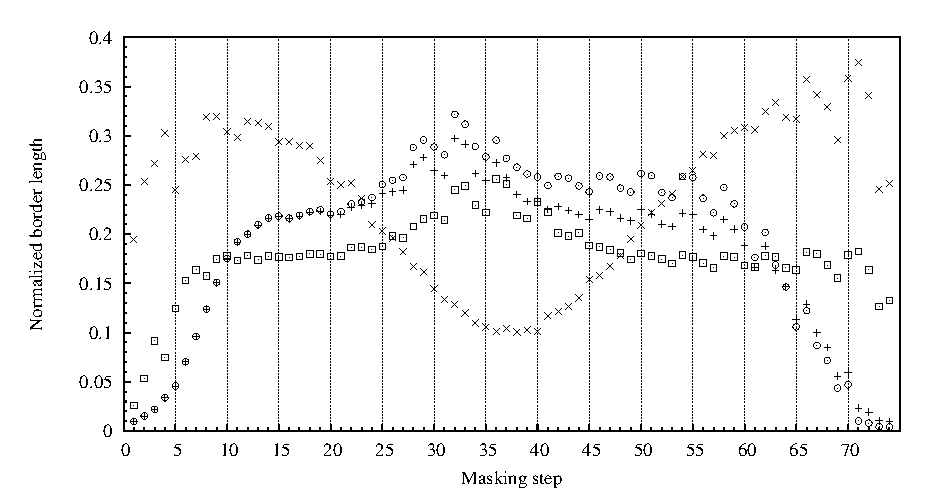
\includegraphics{affy/alternative/EC2}
\caption{\label{fig:alternative_ec2}%
  Normalized border length per masking step of several layouts for the E.\ coli
  Genome 2.0 GeneChip array: original Affymetrix layout with pair-wise left-most
  embeddings ({\tiny $\odot$}), original Affymetrix layout after running two
  passes of a ``pair-aware'' version of Sequential re-embedding ({\tiny $+$}),
  layout produced by \Greedyplus\ with $Q=10$K and Sequential with border length
  minimization ({\tiny $\boxdot$}), and layout produced by \Greedyplus\ with
  $Q=10$K and Sequential with conflict index minimization
  ({\scriptsize $\times$}).}
\end{figure}

%%%%%%%%%%%%%%%%%%%%%%%%%%%%%%%%%%%%%%%%%%%%%%%%%%%%%%%%%%%%%%%%%%%%%%%%%%%%%%%%
\section{Summary}
\label{sec:affy_summary}

We have analyzed the layout of several commercial microarrays with respect to
border length and conflict index. It is clear that placing perfect match (PM)
and mismatch (MM) probes on adjacent spots reduces the incidence of border
conflicts. However, this also has the disadvantage of concentrating the
conflicts on the synthesis steps that add the middle bases, precisely where the
probes are most likely to be damaged.

We have also showed that two algorithms presented in earlier chapters,
\Greedyplus\ and Sequential re-embedding, performed well on real microarrays,
including one of the largest GeneChip arrays available, producing layouts with
up to $8.10\%$ less border conflicts than the original layouts in reasonable
time, and layouts with average conflict index comparable to results on random
arrays. In general, we believe that the quality of currently available GeneChip
arrays can be significantly improved with respect to the problem of unintended
illumination.
